%====================================================================================
\section[Ser \emph{Free rider}]{¿Cuando es racional ser \emph{Free rider}?}
%====================================================================================
\begin{frame}{¿Cuando es racional ser gorrón?}
	Cuando los individuos pueden contribuir sólo positivamente a la provisión del bien público; nadie puede disminuir el nivel de oferta.\\
	
	Cuando la maximización de la utilidad individual puede requerir un pequeño nivel de bien público.
		\begin{align*}
			& \M \limits_{x_B, g_B} \quad U_B\left( x_B, g_A + g_B\right)\\
			& \begin{array}{ll}
				\text{s.a: } & x_B + g_B = w_B, g_B \geq 0
			\end{array}
		\end{align*}
\end{frame}
%------------------------------------------------
\begin{frame}{¿Cuando es racional ser gorrón?}
	\begin{center}
		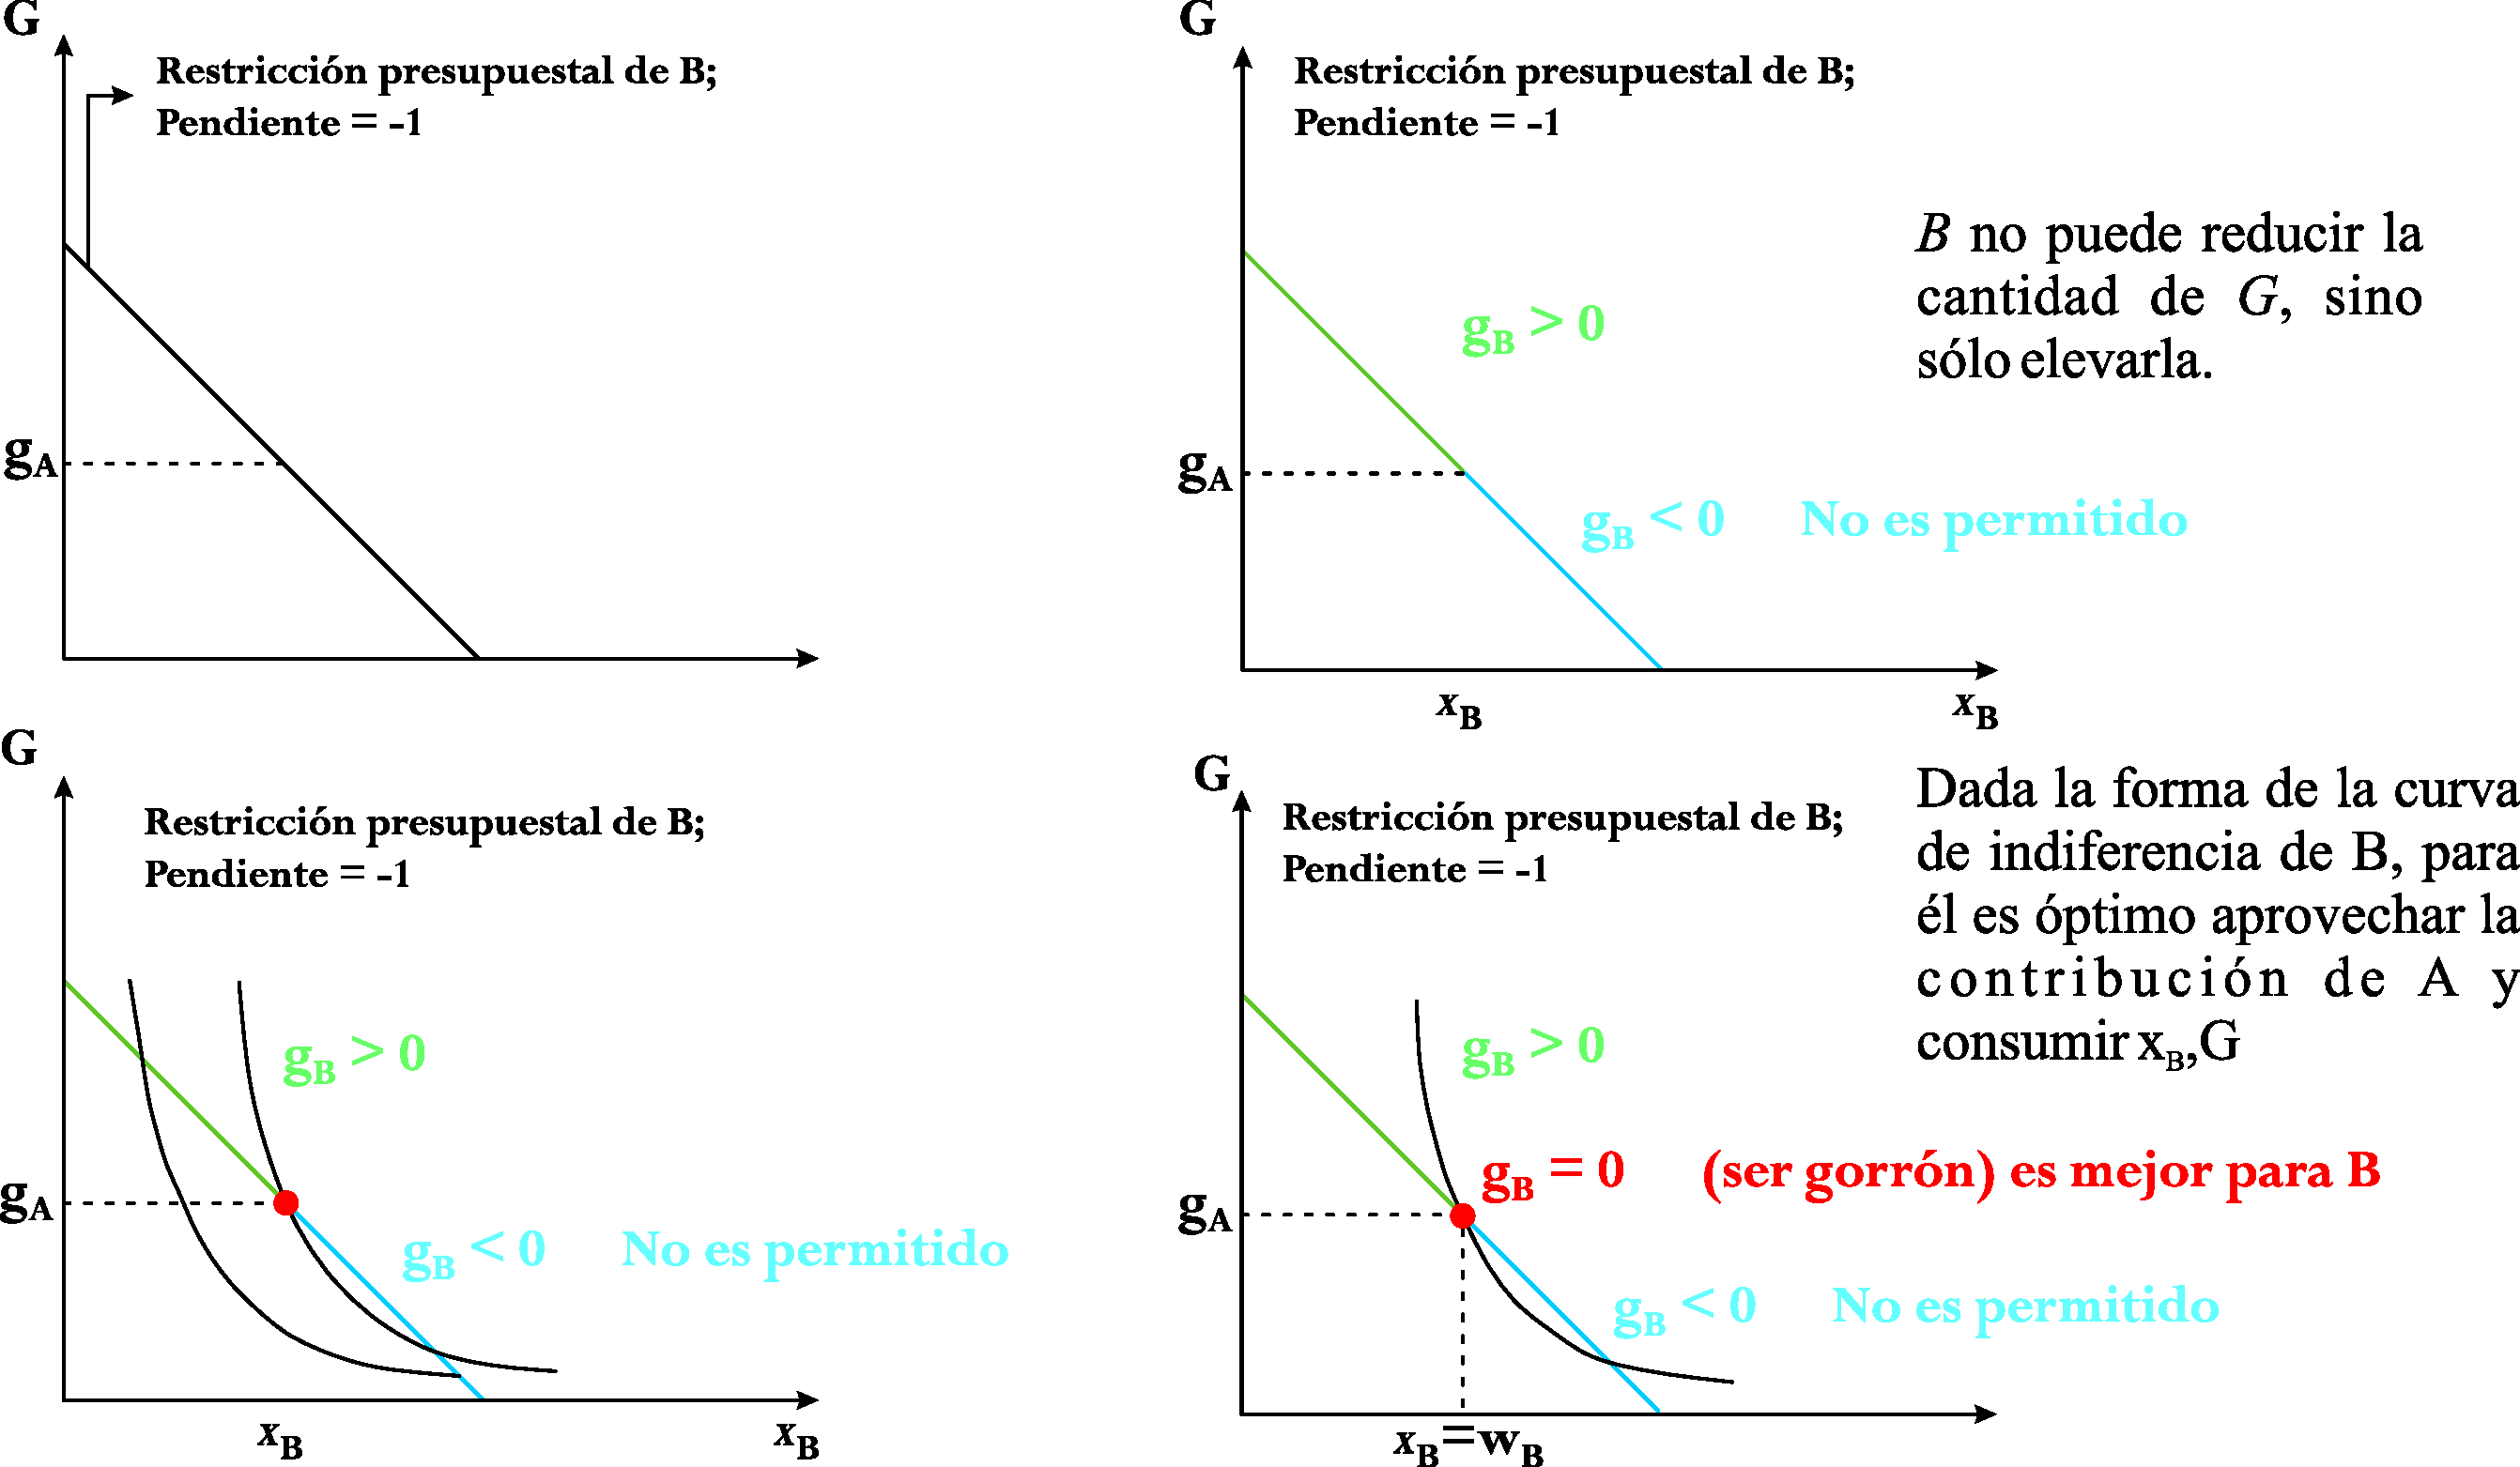
\includegraphics[width = 1\linewidth]{figures/fig_13.pdf}
	\end{center}
\end{frame}